\documentclass[a4paper,11pt]{article}
\usepackage[margin=1in]{geometry}
\usepackage[czech,english]{babel}
\usepackage[utf8]{inputenc} %kodovani
\usepackage[T1]{fontenc}
\usepackage{cmap}
\usepackage{url}
\usepackage{graphicx}
\usepackage{hyperref} 
\usepackage{xcolor}
\hypersetup{
	colorlinks,
	linkcolor={red!50!black},
	citecolor={blue!50!black},
	urlcolor={blue!80!black}
}

\begin{document}

\begin{titlepage}
	\centering
	
\includegraphics[width=0.15\textwidth]{fig/fit-zp2.pdf}\par\vspace{7cm}
	{\scshape\LARGE\bfseries Dopravní telematika\par}
	\vspace{0.5cm}
	{\scshape\Large dokumentace k projektu do předmětu SIN \par}
	\vspace{1.5cm}
	{\huge\bfseries \par}
	\vspace{2cm}
	{\Large\itshape \par}
	\vspace{8cm}
	Filip Denk, XDENKF00
	\\Tomáš Juřica, XJURIC22
\end{titlepage}


\section{TODO}
\begin{itemize}
	\item popsat SUMO
	\item popsat upravování mapy v JOSM (hlavně jaká je s tím jebačka)
	\item jaké je zadání a jaké jsme si dali cíle
	\item co popsat jednotlivá řešení tzn. 2 kruháče a dve křižovatky
	\item popsat výstupy - statistika
	\item přepínání programů řízení - není potřeba, protože se to používá na denní časové úseky a my simulujeme jen hodinovou špičku
	\item dokumentace, napsat do dokumentace, ze vsechny simulace jsou v hodinove spicce, popsat rozpocitane pomery mezi autem/truck/bus a popsat rozdil v cem se lisi (vizualne, accel, decel, ...), nebo vzdalenost mezi auti pri zastaveni
	\item pridat obrazky (graf krizovatky z pdf)
	\item rict ze mame realna data z uradu
\end{itemize}

\begin{figure}[!h]
	\centering
	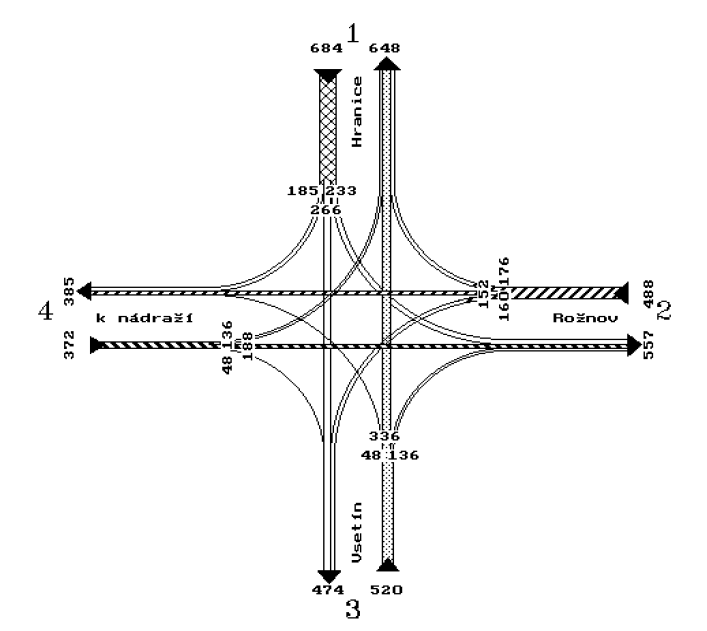
\includegraphics[scale=0.34]{fig/graf.png}
	\caption{fooooo}
	\label{fig:foo}
\end{figure}

\section{Problémy}



\section{Návod ke spuštění}
\subsection{Potřebné prerekvizity}
\begin{itemize}
	\item ...

\end{itemize}


\section{Závěr}


\section{Struktura odevzdaného archivu}
\begin{itemize}
	\item \textbf{foo/bar} - zdrojový kód ...

\end{itemize}

\end{document}
